\documentclass[final]{scrartcl}
\usepackage{graphicx}
\graphicspath{ {./figures/} }
\usepackage{ksgstyle}
\usepackage{listings}
\usepackage{color} %red, green, blue, yellow, cyan, magenta, black, white
\definecolor{mygreen}{RGB}{28,172,0} % color values Red, Green, Blue
\definecolor{mylilas}{RGB}{170,55,241}
\lstset{language=Matlab,%
    basicstyle=\ttfamily\small,
    %basicstyle=\color{red},
    breaklines=true,%
    morekeywords={matlab2tikz},
    keywordstyle=\color{blue},%
    morekeywords=[2]{1}, keywordstyle=[2]{\color{black}},
    identifierstyle=\color{black},%
    stringstyle=\color{mylilas},
    commentstyle=\color{mygreen},%
    showstringspaces=false,%without this there will be a symbol in the places where there is a space
    numbers=left,%
    numberstyle={\tiny \color{black}},% size of the numbers
    numbersep=9pt, % this defines how far the numbers are from the text
    emph=[1]{for,end,break},emphstyle=[1]\color{red}, %some words to emphasise
    %emph=[2]{word1,word2}, emphstyle=[2]{style},    
}


\begin{document}
\pagestyle{empty}

\section{Introduction}
We are currently in the process of cleaning up this repository 
and adding a proper user manual and testing - stay tuned for updates.

\section{Definitions}
\begin{description}
    \item[SOFI] super-resolution optical fluctuation imaging
    \item[Raw data] refers to camera images, saved e.g. as tiff files or in a proprietary format. The pixel gray values are Analog Digital Units (ADU) and include an offset.
    \item[Metadata] is data contained in the raw data that describes the acquisition settings. Additional camera metadata might be required to read in files stored in binary format.\\
    \item[ROI] regions of interest: 
    1. Unless specified, the software divides the camera data into multiple planes and uses the maximal region for each plane. It is possible to crop the maximum common ROI after co-registration of all planes.
    2. Users can specify an ROI in the config file. Only coordinates in this ROI are then used for further analysis.
    \item[Subsequence] the input image sequence is often divided into smaller sequences referred to as subsequences or batches, that are analyzed separately and subsequently averaged.
    \item[SNR] Signal-to-noise ratio
    \item[FRC] Fourier Ring Correlation
    \item[PSF] point spread function
\end{description}

\section{Installation}
\subsection{Quick Start}
    SOFI Analysis Software is developed in Matlab with the core cumulant
    calculation provided for GPU (CUDA) and for CPU (C++ code implemented via Mexx files). 

    The code was tested in Matlab R2016b, under Windows 7, Windows 10 and Mac and requires the XXX toolboxes. No additional software installation is required.

    The following commands will clone the repository
\begin{lstlisting}[language=bash] 
git clone https://github.com/acts-project/acts <source-dir>
\end{lstlisting}

    To launch the calculation:

    1.  Please make sure that test data are in the same folder together with the code.\\ 
    2.  Run \lstinline{multicolor_sofi_main.m}
    
        All tests should pass, results and figures will be saved in the
        automatically created results folder. The analysis of the test data should
        have a runtime of TODO on a standard desktop computer.

\subsubsection*{GPU Version}
    the cumulant calculation can be accelerated by GPU. It requires that the computer has a CUDA-enabled NVIDIA GPU (http://ch.mathworks.com/discovery/matlab-gpu.html).

    If you have the Matlab Parallel Processing Toolbox and a NVIDIA graphics card, write the following command on the "Command Window":
\begin{lstlisting}     
gpuDevice
\end{lstlisting}
    It should display:

\begin{lstlisting}
ans = 
	CUDADevice with properties:
\end{lstlisting}
    with a list of properties. Note the 'ComputeCapibility' of your graphics card.


    Compilation for your GPU card:\\ 
    Step 1: note the 'ComputeCapibility' of your graphics card which is for example '2.0' in the case of NVIDIA Geforce GTX 480. 
    The compute capability of a graphics card can also be found here: https://developer.nvidia.com/cuda-gpus\\
    Step 2: Set the Matlab current folder to \lstinline{multicolor_sofi\funcs\private}. The tab "Current folder" should display files including 'gpu.cu', 'gpu.ptx', 'nvcc.m' and 'nvccbat.bat'.\\
    Step 3: Execute the following command on the "Command Window": 
\begin{lstlisting}
nvcc -arch=sm_20 -ptx gpu.cu
\end{lstlisting}
    This command launches the NVIDIA compiler to recompile gpu.cu. Make sure that the -arch option is set to the compute capability of your CUDA-capable graphics card. In the example displayed above, it is 2.0 (the compute capibility of NVIDIA Geforce GTX 480).

\subsubsection*{CPU Version}
    We recommend using the GPU version of the SOFI algorithm (see above). The Mexx
    files included in the current software package are compiled for Win32bit
    systems and we provide the original files that the user can compile for their
    computer system.

\section{Overview of SOFI processing}
brief overview of theory e.g. from Self-Blinking Dyes Unlock High-Order and Multiplane Super-Resolution Optical Fluctuation Imaging https://doi.org/10.1021/acsnano.0c04602 or from SOFI simulation tool: A software package for simulating and testing super-resolution optical fluctuation imaging 10.1371/journal.pone.0161602

\subsection{2D SOFI Workflow}
adapt illustration from Mapping molecular statistics with balanced super-resolution optical fluctuation imaging (bSOFI) 10.1186/2192-2853-1-4 
\subsection{Cross-cumulant calculation}
adapt illustrations
\begin{figure}[h]
  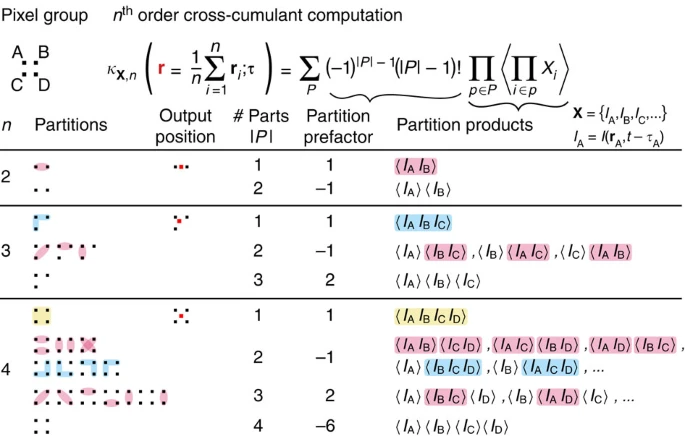
\includegraphics[width=0.5\linewidth]{cross-cumulantCalculation.png}
  \caption{Cross-cumulant calculation Live-cell multiplane three-dimensional super-resolution optical fluctuation imaging 10.1038/ncomms6830}
  \label{fig:CCC}
\end{figure}

\begin{figure}[h]
  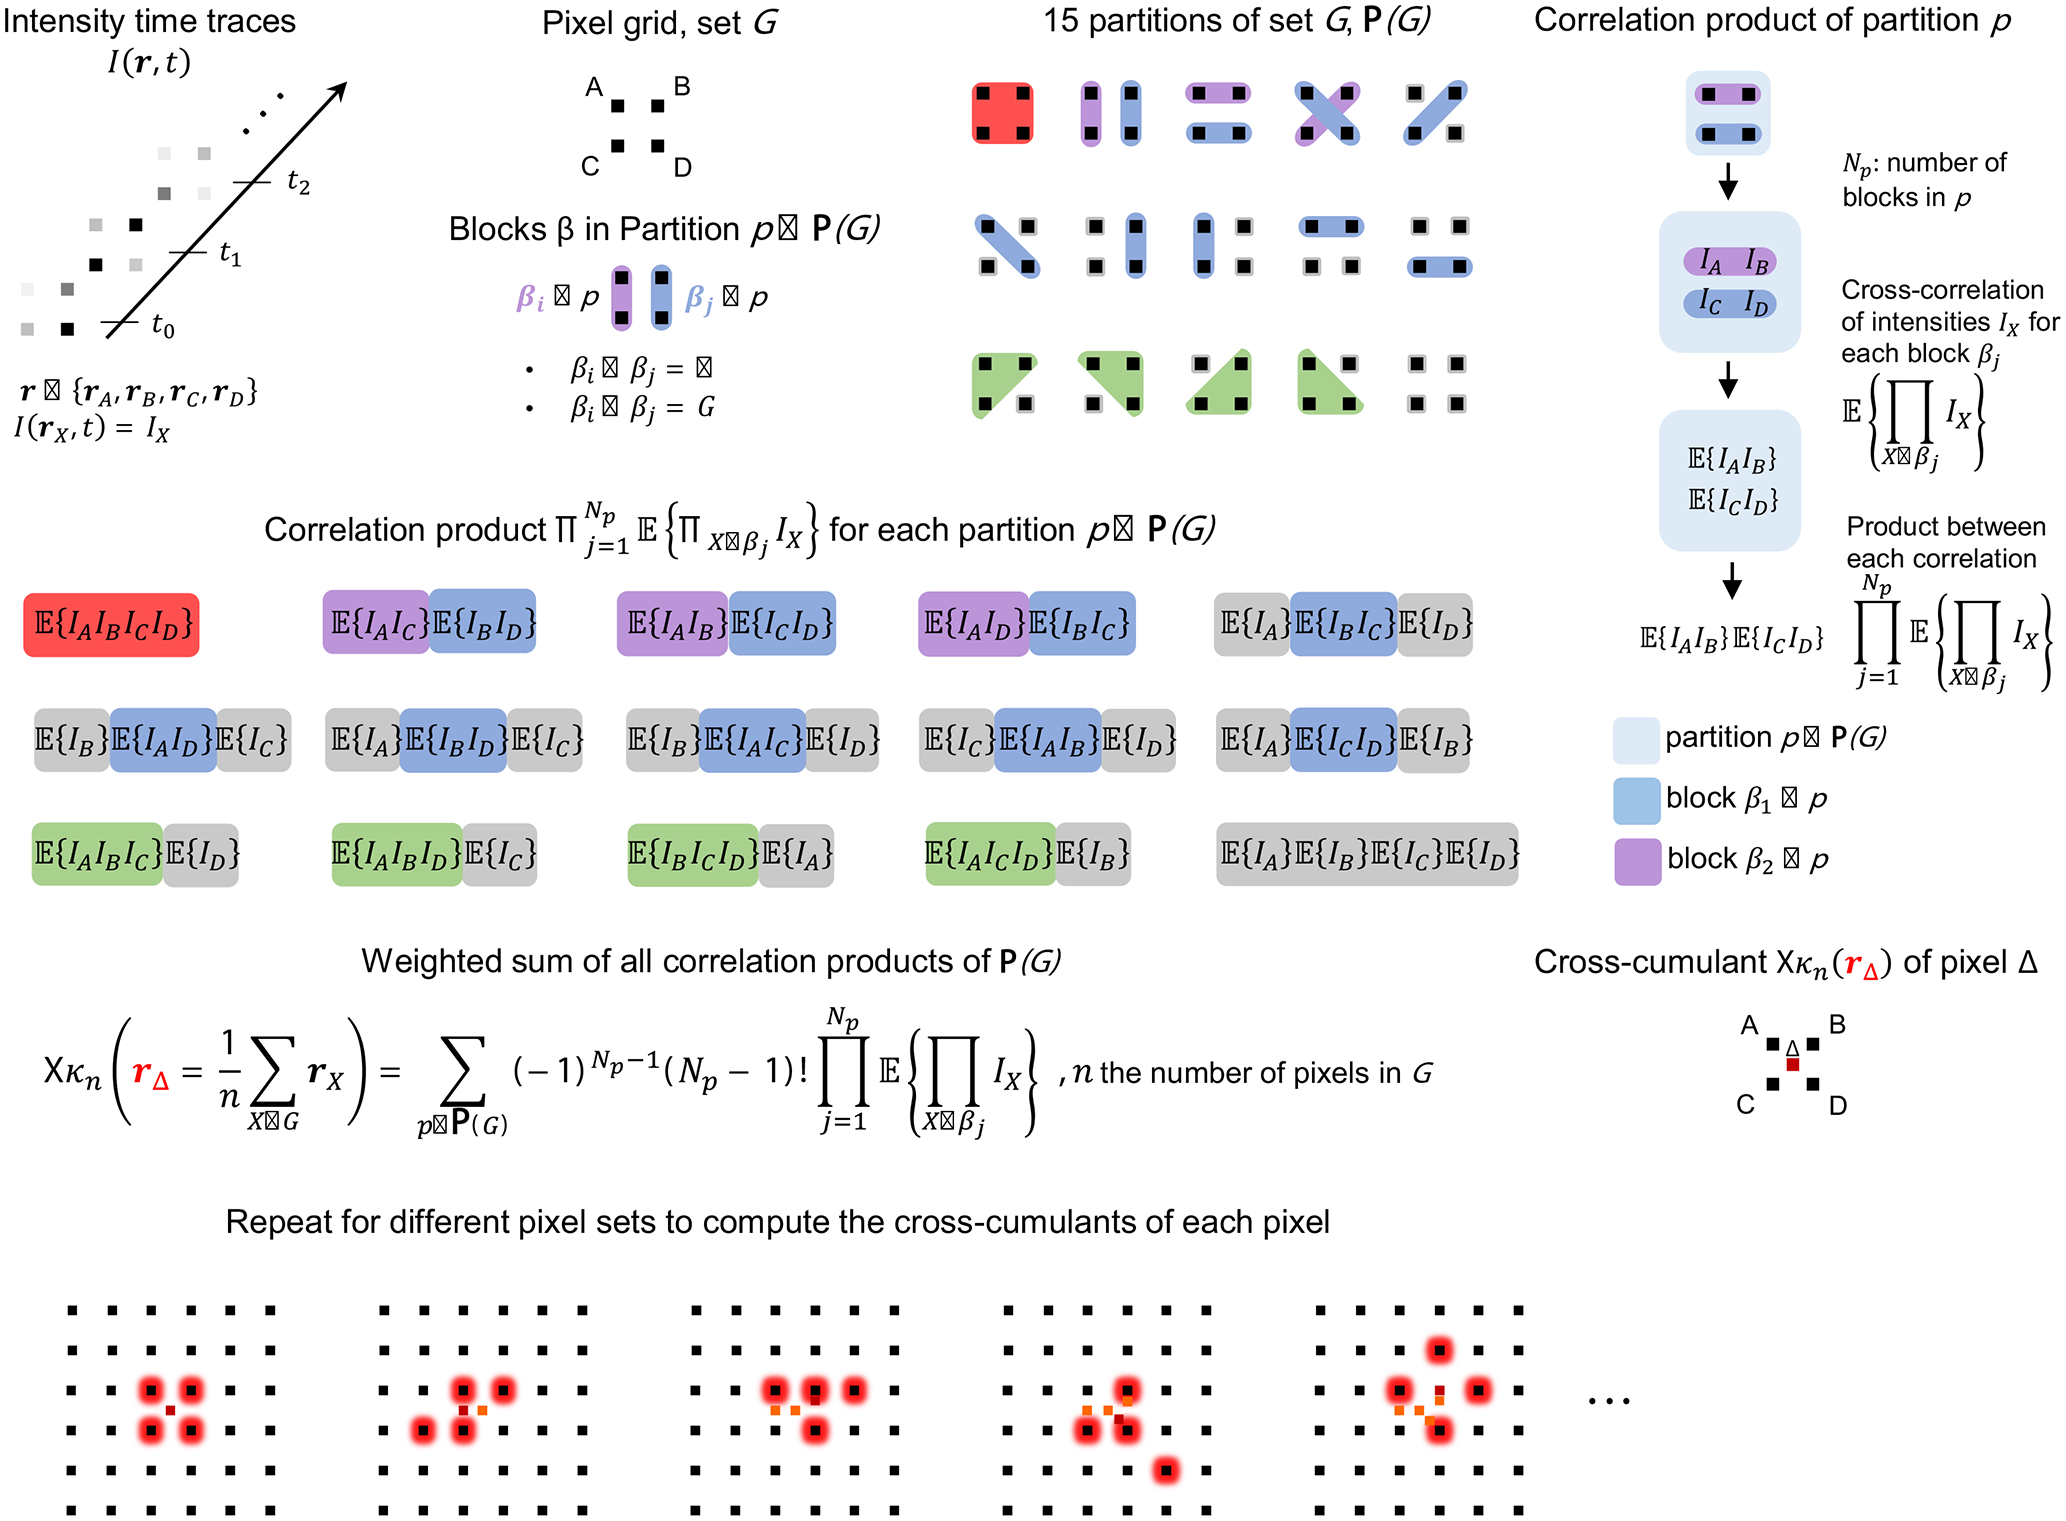
\includegraphics[width=0.8\linewidth]{pone.0161602.g003.PNG_L.png}
  \caption{Cross-cumulant calculation SOFI simulation tool: A software package for simulating and testing super-resolution optical fluctuation imaging 10.1371/journal.pone.0161602}
  \label{fig:CCC}
\end{figure}

\subsection{3D SOFI Workflow}

\begin{figure}[h]
  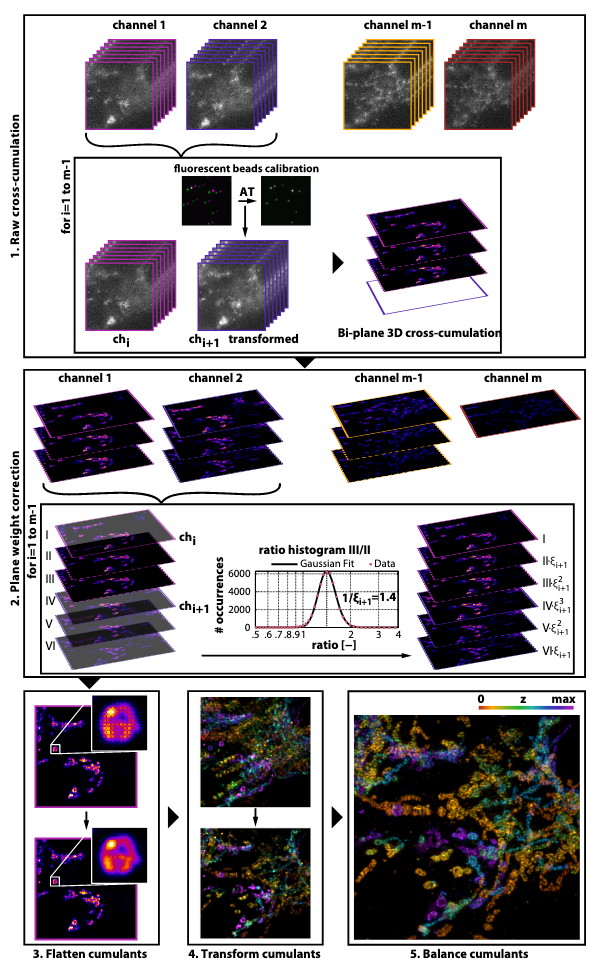
\includegraphics[width=0.7\linewidth]{multiplaneWorkflow.png}
  \caption{multiplane workflow Live-cell multiplane three-dimensional super-resolution optical fluctuation imaging 10.1038/ncomms6830}
  \label{fig:CCC}
\end{figure}

\begin{figure}[h]
  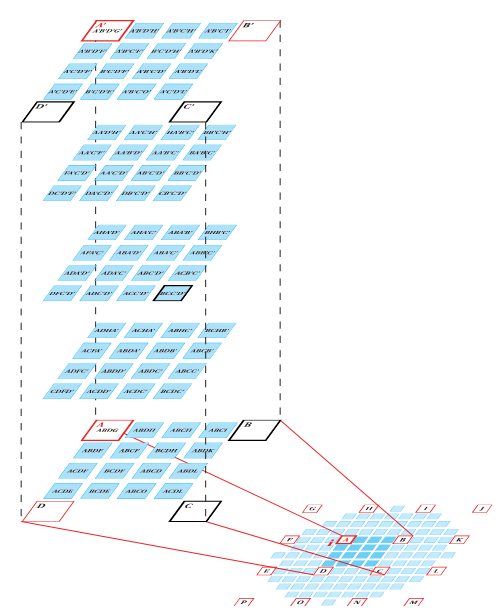
\includegraphics[width=0.5\linewidth]{4thOrderMultiplaneCumulant.png}
  \caption{Cross-cumulant calculation 3D Live-cell multiplane three-dimensional super-resolution optical fluctuation imaging 10.1038/ncomms6830}
  \label{fig:CCC}
\end{figure}

\subsection{SOFI processing options explained}

All the processing options are set in the config file and are briefly explained in the following.
\subsubsection*{Input settings and preprocessing}
These settings let you control which data files will be processed; typically we provide the path to the folder that contains all the measurements and specify the file type by providing the file extension. The software will select all corresponding data in the folder. Currently, reading of tiff files up to 4Gb and binary data files is supported. For binary data files, the image width and height need to be supplied in pixels. It is possible to specify a region of interest that should be analyzed. Optionally, consecutive files with the same core file name and a different numbering can be concatenated into one.

\begin{lstlisting}[language=Matlab] 
% INPUT SETTINGS
% path to data files - folder with all the measurements to process
str = '.raw';
% (.tif, .tiff, '.dat', '.raw') specify the file type by the file extension, 
% currently reads original tif(f) files up to 4Gb
% for bigger files load_bigtif often failes, try imread_big?
settings.io.imagePath = 'H:\Vytautas_data_for_Klaus_2021\Vytautas_2021_01_07\SNR_estimation_with_JK\DATA';
settings.io.fext = str;
settings.io.W = 400;
settings.io.H = 400;
fnames = getnamesdir(settings.io.imagePath, str)'; % search for the file names automatically

settings.io.roi = []; % ROI to be loaded, drift and bleach corrected- keep empty [] if the whole image should be used
settings.io.roisx = {}; % ROI (image colums) to be processed by SOFI (example "settings.io.roisx = {61:360}")
settings.io.roisy = {}; % ROI (image rows) to be processed by SOFI (example "settings.io.roisy = {61:360}")

%%% CHECK/ADJUST IMAGE PROCESSING SETTINGS

% Preprocessing settings
settings.io.ro = 0; % reorder Nikon data (DNA data from Leuven)
settings.io.figs =1; % create figures yes/no {1,0}
settings.io.figformat = 'png'; % figure will be saved in the specified format {'fig','png','pdf'}
settings.io.figshow =0; % show figures yes/no {1,0}
settings.io.figsave =1; % save figures (which figures - please explain difference in scaling) yes/no {1,0}
settings.io.matsave =0; % save results (what results?) in matfile (can take a lot of memory on the drive)
settings.io.concatOn =0; % concatenate consecutive images yes/no {1,0} TODO: needs better explanation!
settings.io.concatSave =0; % save concatenate images in one file yes/no {1,0} TODO: needs better explanation!
\end{lstlisting}

\subsubsection*{Output settings}
These settings let you control where the SOFI results will be stored; typically we use the path to the folder that contains all the measurements and append the most important processing options to the folder name.
After code rearrangement, there should be a more uniform naming convention for the results. For 2D processing we provide e.g. bleaching curves and molecular parameter estimate files in a seperate folder, SOFI results are directly saved and have respective file endings: _CX raw cumulants with X cumulant order, _SOFIX for standard processing or _SOFI_linX for adaptive linearization

\begin{lstlisting}[language=Matlab]
% OUTPUT SETTINGS 
mname = fnames{1};
settings.io.outputpath = settings.io.imagePath; 
%     num2str(settings.io.blcor ),'dc',num2str(settings.io.dcor),'_start',num2str(settings.sys.start)];% output folder for results
% if ~isempty(settings.sys.sub)
settings.io.outputpath = [settings.io.outputpath,'_', settings.dec.deconv_method,'_FWHM', num2str(settings.dec.fwhm), '_iter',num2str(settings.dec.iter),'_recon',num2str(settings.dec.reconvolve), '_wsize', num2str(settings.sys.wsize), ...
    '_start', num2str(settings.sys.start), '_end', num2str(settings.sys.end)];    
settings.io.bits = 16; % number of bits of the output tif file {8,16}
\end{lstlisting}

\subsubsection*{Cumulant calculation}
These settings offer control about which cumulant orders are calculated and which frames are evaluated (start..stop) and until which frame the data is read (sub). wsize is the subsequence size, i.e. the data is divided into chunks of wsize frames, processed and all subsequences are averaged. This is a popular way to suppress the influence of photobleaching on cumulant analysis (anything introducing correlations will result in SOFI signal, but not necessarily contribute to enhancing the resolution see Smoothness correction for better SOFI imaging https://www.nature.com/articles/s41598-021-87164-4). wsize should be significantly smaller (5 times) smaller than the photobleaching halftime, but need to allow sufficient sampling of blinking statistics. Maybe we can move this to the bleaching correction section?

\begin{lstlisting}[language=Matlab]
% Cumulant calculation settings
settings.sys.orders = 1:4;
settings.sys.wsize = 1000; % substack for analysis to avoid correlations from bleaching etc
settings.sys.sub = [];%[550];%10050%[20000]; % evaluate only first n frames (for quick preview)
settings.sys.start = []; %51; start from frame start; if empty, it starts from the first frame
settings.sys.end = []; % end at frame end; if empty, it reads until the last frame
\end{lstlisting}

\subsubsection*{Drift correction}
We provide different options for drift correction. Obviously, drift will result in a loss of correlation. In our experience, drift correction based on cross-correlation between the different SOFI subsequences id often precise enough (option SOFI). If available, drift correction based on fiducial markers is more precise. You can supply e.g. such a file created in ThunderSTORM ImageJ plugin or from \lstinline{LBEN_PALM} Matlab codes. The latter options have not been used for a while.

\begin{lstlisting}[language=Matlab]
% Drift correction settings TODO: please check explanation and complete it!
settings.io.dcor = 1;% turn on or off drift correction, if on
% - specify path to drift correction file if drift correction method is other than SOFI
settings.dcor.type = 'SOFI'; % drift correction method {'TS','LBEN_PALM','SOFI'}
% We assume the drift correction file to be : [settings.io.imageFile,settings.dcor.tag]
settings.dcor.tag = '_drift';%'driftcor'; % additional tag for drif corr. file {_drift_corr, drift,driftcor}
% TS: drift correction based on ThunderSTORM .json file (either from fiducial markers or cross-correlation)
% LBEN_PALM:
% SOFI: first cross-correlation between 100 frames subsequences (why not variable?) and first 100 frames, performed for mean of stack??
% then followed by cross-correlation between first and other SOFI2
% subsequences (is this the same as in biplane?)
\end{lstlisting}

\subsubsection*{Bleaching Correction}
This intends to fit the average fluorescence intensity over time using an exponential function and corrects the data to suppress the unwanted correlations from photobleaching. Should be replaced in the future by the approach in Smoothness correction for better SOFI imaging https://www.nature.com/articles/s41598-021-87164-4.

\begin{lstlisting}[language=Matlab]
% Bleaching correction settings
settings.io.blcor = 1; % bleaching correction off/on {0,1}
settings.blcor.type = 'monoexp';%'monoexp'; % {monoexp, iir}
settings.blcor.MaxCorrSamp = 5000; % TODO: needs better explanation!
\end{lstlisting}

\subsubsection*{Deconvolution Options}
It is optional to deconvolve, linearize (two outputs for 2D data: standard sqrt or adaptive linearization) and reconvolve the raw cumulants.
We implemented different options for deconvolution. The standard is Lucy-Richardson deconvolution with a Gaussian psf. You can define the psf FWHM in pixels and specify the number of iterations..don't overdue it we usually use 5-10 iterations but this needs to be finetuned for each dataset and checked for artifacts and overdeconvolution. For LR it is also possible to use an Airy-function as a psf model. Since LR has a positivity constrained it is not the optimal deconvolution algorithm. Two other algorithms based on Bregman/augmented lagrangian deconvolution can be used (GPU and CPU implementation) and are better for low signal-to-noise data. This has not been published in detail, but is described in the thesis of Tomas Lukes. Needs more explanation on parameter choices.

\begin{lstlisting}[language=Matlab]
    % POST PROCESSING SETTINGS

    % TODO: which part is this used for?
    settings.sys.pxy = 108; % projected pixel size (in xy) [nm]  sofisetup = 96.0384, Hendriksetup = 104.8, AD-gut setup = 108

    % Deconvolution/Linearization settings
    settings.dec.deconv_method = 'lucy'; % {'breg_cuda', 'augLag_mb', 'lucy'}
    settings.dec.fwhm = 3;
    settings.dec.lin = 1; % option to turn on/off linearization
    settings.dec.reconvolve = 0; % option to turn on/off reconvolution using 
    % conv and the theoretical psf model "airy", or "gaussian" chosen below
    settings.dec.denoise = 1; % only applies to SOFI lin

    % parameters for Lucy-Richardson deconvolution
    settings.dec.iter = 5;
    settings.dec.psfmodel = 'gaussian';% choice of theoretical "airy", or "gaussian"

    % parameters for cuda version of bregman iterative method based
    % deconvolution with Gaussian noise model and Gaussian psf model
    settings.bregman.iter = 10;
    settings.bregman.apodize =0;
    settings.bregman.lambda = 0.03;
    settings.bregman.omega = 0.95;
    settings.bregman.NumImages = 1;

    % parameters for matlab version of augmented lagrangian based deconvolution
    % with Gaussian noise model and Gaussian psf model
    settings.augLag.gamma = 2000;
    settings.augLag.beta = settings.augLag.gamma;
    settings.augLag.alpha = 1;
    settings.augLag.reltol = 1e-4;
    settings.augLag.maxIter = 3;
    settings.augLag.Lp = 1;
    % settings.augLag.Lp = 1; % defines which Lp norm to use (hardcoded to 1 in
    % the code)
    
\end{lstlisting}

\subsubsection*{Molecular Parameter Estimation}
Using three different SOFI orders and/or estimation of the on-time the molecular density, the on-time ratio of the fluorophore blinking kinetics and the molecular brightness is possible Mapping molecular statistics with balanced super-resolution optical fluctuation imaging (bSOFI) 10.1186/2192-2853-1-4 or Complementarity of PALM and SOFI for super-resolution live-cell imaging of focal adhesions https://doi.org/10.1038/ncomms13693. 
\begin{lstlisting}[language=Matlab]
% Molecular parameters
settings.molpar.run = 1; % turn on or off
settings.molpar.thresh = 0.1; % TODO: needs better explanation!
% please add an option for saving in .mat file and .tif
% use tirf yes/no as option for brightness calculation
\end{lstlisting}

\subsubsection*{On-time Estimation}
Using a second-order cumulant (same as cross-correlation) analysis with varying lag-time, the blinking can be analyzed and under certain conditions the on-time ratio can be easily determined using an exponential fit - this is basically FCS. Mapping molecular statistics with balanced super-resolution optical fluctuation imaging (bSOFI) 10.1186/2192-2853-1-4.
\begin{lstlisting}[language=Matlab]
% Estimate Ton
settings.ton.run = 1; % turn on or off
settings.ton.wsize = 300;
settings.ton.numtau = 20; % TODO: needs better explanation!
\end{lstlisting}

\subsubsection*{Jacknife SNR Estimation}
This enables estimation of the signal-to-noise ratio using Jacknife resampling and is SOFI specific. The algorithm is computationally expensive. More information can be found in Complementarity of PALM and SOFI for super-resolution live-cell imaging of focal adhesions https://doi.org/10.1038/ncomms13693 and Model-free uncertainty estimation in stochastical optical fluctuation imaging (SOFI) leads to a doubled temporal resolution doi:10.1364/BOE.7.000467.
\begin{lstlisting}[language=Matlab]
% Jacknife SNR estimation
settings.sys.jk = 1; % turn on/off the Jacknife SNR estimation - where is it in the code?
settings.jk.orders = 1:4;
settings.sys.block = 1; % TODO: needs better explanation!
\end{lstlisting}

\subsubsection*{FRC Resolution Estimation}
SOFI specific implementation of Fourier-Ring correlation to estimate the image resolution, see Complementarity of PALM and SOFI for super-resolution live-cell imaging of focal adhesions https://doi.org/10.1038/ncomms13693. Will probably be removed from the code as we recommend decorrelation analysis for resolution estimation. We should keep a paragraph on how to estimate the resolution, maybe also link to some information from SOFIevaluator: a strategy for the quantitative quality assessment of SOFI data https://doi.org/10.1364/BOE.382278
\begin{lstlisting}[language=Matlab]
% FRC calculation
settings.frc.run = 0; % turn on or off
settings.frc.orders = 1:3;
settings.frc.bcgsub = 1;%1.3;
settings.frc.pixelsize = settings.sys.pxy; % projected pixel size (in xy) [nm]  sofisetup = 96.0384, Hendriksetup = 104.8, AD-gut setup = 108
    
\end{lstlisting}

\subsection{Multicolor SOFI}
To be inserted once the codes have been merged. See Spectral cross-cumulants for multicolor super-resolved SOFI imaging https://doi.org/10.1038/s41467-020-16841-1  

\end{document}
